\documentclass[10pt, notitlepage]{article}
  \usepackage[utf8]{inputenc}		%UTF-8 kodovanie
  \usepackage[czech]{babel}				%cestina
  \pagestyle{empty}								%bez cislovania stran
  \usepackage{graphicx}						%na obrazky
  \usepackage{wrapfig}						%na obtekanie obrazkov
  \usepackage{amsmath}						%matematicke prostredie
  \usepackage{amssymb}						%matematicke fonty
  \usepackage{eucal}							%matematicke fonty
  \usepackage{epstopdf}						%matematicke fonty
  %\usepackage{wasysym}						%nejake dalsie znaky ... na smajlika v priklade 34zima11
  \usepackage[a4paper, left=1.5cm, bottom=0cm, top=1cm, right=3.3cm]{geometry}%okraje stranky
  %\usepackage[table]{xcolor}			%farebne tabulky ... na tmave miesta v tabulkach
  \usepackage{comment}
  \usepackage{color}
  \usepackage{qrcode}
  
  %\def \reseni{1}% zakomentovat pro tisk zadani
  \def \ifzadani{\ifx\reseni\undefined}
  
  
  \def \cislotymu {42}%%{##CISLO_TYMU##}
  %\def \cislotymu {\ }
  \qrset{height=1cm}
  \def \printcislotymu {\llap{\it(\cislotymu) \qquad}}
  
  
  %prikaz pre vytvorenie prikladu, ktory sa nebude rozdelovat na 2 strany
  %s defaultnou medzerou 2cm medzi prikladmi
  %priklady su cislovane automaticky
  %vsetky priklady spolu vlozit do prostredia \begin{enumerate} \end{enumerate}
  %prikazom \priklad{text a prislusenstvo prikladu}
  %prvy parameter je zadanie prikladu
  %druhy parameter je vysledok prikladu
  %medzi moznostami s/bez vysledkov sa prepina dvoma riadkami oznacenymi komentarmi
  %riadok sa vypne napisanim % na zaciatok riadku
  \newcommand{\priklad}[2]{
    \begin{minipage}{\textwidth}
    \item \noindent \printcislotymu \raisebox{0pt}[0pt][0pt]{\llap{\raisebox{-5.3ex}{\qrcode{T\cislotymu P\number\numexpr\value{enumi}\relax} \enskip}}}#1
    \ifzadani
        \vspace{45pt}
    \else
        \begin{flushright}\vspace{-6pt} [$\,$#2$\,$]\vspace{28pt}\end{flushright}
    \fi
    \end{minipage}}
  
  %priklad s obrazkom, zadava sa v tvare: \prikladsobrazkem{zadanie}{riesenie}{adresa obrazka}{cast, ktoru ma obrazok zaberat z celej sirky textu, cislo od 0 do 1}{1-predosle cislo}
  
  \newcommand{\prikladsobrazkem}[5]{
    \begin{minipage}{\textwidth}  
      \begin{minipage}[l]{#5\textwidth}
      \item \noindent \printcislotymu \raisebox{0pt}[0pt][0pt]{\llap{\raisebox{-5.3ex}{\qrcode{T\cislotymu P\number\numexpr\value{enumi}\relax} \enskip}}}#1
    \end{minipage}\hspace{0.05\textwidth}
    \begin{minipage}[r]{#4\textwidth}
  %	  \vspace{-40pt}
      \begin{center}
        \includegraphics[width=\textwidth]{#3}
      \end{center}
    \end{minipage}
      \ifzadani
        \vspace{45pt}
      \else
      \begin{flushright}\vspace{-6pt}[$\,$#2$\,$]\vspace{28pt}\end{flushright}
      \fi
    \end{minipage}}
  %vlozenie obrazka
  %obrazok sa vlozi prikazom \obrazek{nazov suboru obrazku napr.: trojuholnik.eps}{sirka obrazku}
  \newcommand{\obrazek}[2]{
    \begin{wrapfigure}{r}{#2}
      \vspace{-40pt}
      \begin{center}
        \includegraphics[width=#2]{#1}
      \end{center}
    \end{wrapfigure}}
  %pripadne urcenie velkosti moze byt dalsi parameter, alebo ak su vsetky obrazky to scale, moze sa hranata zatvorka
  %uplne vypustit
  
  \begin{document}
  \begin{enumerate}
  \renewcommand\labelenumi{\bfseries\theenumi.}
  
  
  \priklad{Čtyři kolegové si rozdělili výdělek následujícím způsobem: první dostal pětinu částky, zbývající tři si rozdělili zbytek na tři stejné části. V jakém poměru jsou výdělky prvního a druhého kolegy v tomto pořadí?}{3:4}
  
  %%%%%%%%%%%%%%%%%%%%%%%%%%%%%%%%%%%%%%%%%%%%%%%%%
  
  \priklad{Čtvrtkruh s poloměrem 4 má stejně velký obsah jako kruhová výseč o poloměru 3. Jaká je velikost středového úhlu výseče?}{$160^\circ $}
  
  %%%%%%%%%%%%%%%%%%%%%%%%%%%%%%%%%%%%%%%%%%%%%%%%%
  
  \priklad{V jedné továrně řádí chřipková epidemie, takže na noční službě se střídají pouze čtyři pracovníci. Kolik nocí v řadě už odsloužil Adam? Víme, že už odsloužil více než Bedřich, který zvládl jen čtyři noci. Naopak Cyril už pracoval 15 nocí po sobě, což je dokonce víc než Adam a Bedřich dohromady. A pak je tu ještě David, který odsloužil sice méně než Adam, ale i tak to bylo už 9 nocí.}{10 nocí}
  
  %%%%%%%%%%%%%%%%%%%%%%%%%%%%%%%%%%%%%%%%%%%%%%%%
  
  \priklad{Honza má stejně sester jako bratrů, ale jeho sestra má dvakrát více bratrů než sester. Kolik je v této rodině hochů a děvčat, pokud počítáme jen nejmladší generaci?}{4 hoši a 3 děvčata}
  
  %%%%%%%%%%%%%%%%%%%%%%%%%%%%%%%%%%%%%%%%%%%%%%%%
  
  \priklad{Výrobek byl zlevněn o $ 8\% $ a stojí tak nyní 299 Kč. Kolik stál před slevou?}{325 Kč}
  
  %%%%%%%%%%%%%%%%%%%%%%%%%%%%%%%%%%%%%%%%%%%%%%%%%
  
  \priklad{Petr rozřezal dvě tyče na stejné, ale co největší možné díly. Jedna tyč měřila $ 42\,cm $, druhá $ 63\,cm $. Kolik dílů získal Petr a jak byly díly dlouhé?}{5 dílů po $ 21\,cm $}
  
  %%%%%%%%%%%%%%%%%%%%%%%%%%%%%%%%%%%%%%%%%%%%%%%%%
  
  \priklad{Myslím si přirozené číslo. Když ho vynásobím čtyřmi, vzniklé číslo pak zvětším o jeho tři čtvrtiny, výsledek zvýším o jedna a pak vydělím devíti, k tomu přičtu dvojku, výsledek zdvojnásobím, celou sumu vynásobím samu sebou, vzniklou mocninu zmenším na setinu, od toho odečtu sedm, ze zbytku udělám druhou odmocninu a tu zvýším o dvě, dostanu číslo pět. Jaké číslo si myslím?}{23}
  
  %%%%%%%%%%%%%%%%%%%%%%%%%%%%%%%%%%%%%%%%%%%%%%%%%%
  
  \priklad{Mošt se prodává v 5litrových a 2litrových lahvích. Pan Suchánek skoupil celkem $ 216\,l $ moštu v 60 lahvích. Kolik litrů moštu si pan Suchánek koupil v 5litrových láhvích? Víme, že všechny zakoupené láhve byly plné.}{$ 160\,l $}
  
  %%%%%%%%%%%%%%%%%%%%%%%%%%%%%%%%%%%%%%%%%%%%%%%%%%%%%%%
  
  \priklad{Ve fitcentru si vedou měsíční statistiky. Dvě pětiny návštěvníků chodí do fitcentra alespoň dvakrát týdně, osmina z nich dokonce denně. Čtvrtina návštěvníků chodí jedenkrát týdně. Každá dvacátá osoba se po první návštěvě fitcentra vícekrát nevrátí. Zbytek návštěvníků chodí několikrát do měsíce, ale nepravidelně. Kolik procent návštěvníků chodí do fitcentra pravidelně?}{65\%}
  
  %%%%%%%%%%%%%%%%%%%%%%%%%%%%%%%%%%%%%%%%%%%%%%%%%%%%%%%
  
  \priklad{Sandra má v knihovně 9 nepřečtených knížek a na dovolenou si chce vzít právě 2 z nich. Kolika způsoby si je může vybrat?}{36}
  
  %%%%%%%%%%%%%%%%%%%%%%%%%%%%%%%%%%%%%%%%%%%%%%%%%%%%
  
  \priklad{Podle jízdního řádu má být vlak za 10 minut ve stanici. K nádraží mu ale zbývá ještě $ 32\,km $. Vlak za~každé 2 minuty ujede $ 3\,km $, kromě posledního dvoukilometrového úseku, který mu bude trvat 5 minut. Jaké zpoždění se objeví ve stanici na informační tabuli?}{15 minut}
  
  %%%%%%%%%%%%%%%%%%%%%%%%%%%%%%%%%%%%%%%%%%%%%%%%%%%%%%
  
  \priklad{Pozemek tvaru obdélníku má výměru $ 300\,m^2 $. Jedna jeho delší strana je ohraničena řekou, pouze tři zbývající strany jsou oploceny. Délka plotu je $ 49\,m $. Jaké jsou rozměry pozemku?}{$ 25\,m\times12\,m$  nebo  $24\,m \times 12{,}5\,m $}
  
  %%%%%%%%%%%%%%%%%%%%%%%%%%%%%%%%%%%%%%%%%%%%%%%%%%%%%%%
  
  \priklad{Určete v základním tvaru postupný poměr $ \alpha:\beta:\gamma:\delta $ velikostí vnitřních úhlů rovnoběžníku $ ABCD $ , je-li $ \gamma=55^\circ $.}{$ 11 : 25 :11 : 25 $}
  
  %%%%%%%%%%%%%%%%%%%%%%%%%%%%%%%%%%%%%%%%%%%%%%%%%%%%%%%
  
  \priklad{O pěti kamarádech Brunovi, Davidovi, Gustovi, Jáchymovi a Richardovi víme toto:
    \begin{itemize}
    \item Muž, který pije rád kávu a hraje šachy, není ani Richard ani Jáchym. 
    \item Ten, jehož koníčkem je divadlo, je hrnčíř.
    \item Farmářovým koníčkem je hra na housle a určitě to není David, o kterém víme, že má rád mléko.
    \item Gusta, který má rád džus, také není farmářem.
    \item Muž, jehož koníčkem je běh, nepije rád minerálku.
    \item Richard je kuchařem a rád si pochutná na kvalitním čaji.
    \item Bruno ani Gusta nejsou učiteli.
    \item Jeden z kamarádů je horník.
    \item Koníčkem jednoho z přátel je plavání.
    \end{itemize}
  Jakou práci vykonává David?}{učitel}
  
  %%%%%%%%%%%%%%%%%%%%%%%%%%%%%%%%%%%%%%%%%%%%%%%%%%%%%
  
  \priklad{Maruška přinesla na oslavu narozenin své nejlepší kamarádky 320 zákusků 4 druhů: věnečky, indiánky, kremrole a rolády. Věnečků bylo třikrát více než indiánků, indiánků bylo třikrát víc než kremrolí a kremrolí bylo třikrát více než rolád. Kolik kusů rolády Maruška přinesla?}{8}
    
  %%%%%%%%%%%%%%%%%%%%%%%%%%%%%%%%%%%%%%%%%%%%%%%%%%%%
  
  \priklad{Najděte nejmenší přirozené číslo $ c $ takové, aby nejmenší společný násobek čísel 42, 12 a $ c $ byl 252.}{9}
  
  %%%%%%%%%%%%%%%%%%%%%%%%%%%%%%%%%%%%%%%%%%%%%%%%%%%%%
  
  %\prikladsobrazkem{Jak bude vypadat trojrozměrné těleso, pokud znáte jeho bokorys, nárys (pohled zepředu) i půdorys?}{cojeto}{arg3}{0.5}{0.5}
  
  %%%%%%%%%%%%%%%%%%%%%%%%%%%%%%%%%%%%%%%%%%%%%%%%%%
  
  \priklad{Rovnoběžník je sestaven ze čtyř shodných rovnoramenných trojúhelníků. První trojúhelník je obarven ze 40\%, druhý je obarven celý, třetí ze $ 2/3 $ a poslední ze $ 13/30 $. Vyjádřete ve zlomku v základním tvaru, jak velká část rovnoběžníku je obarvena.}{$ 5/8 $}
  
  %%%%%%%%%%%%%%%%%%%%%%%%%%%%%%%%%%%%%%%%%%%%%%%%%%%%%%
  
  \priklad{Když 6 švestek a 1 jablko má hodnotu 1 hrušky a 3 jablka s 1 hruškou mají hodnotu 10 švestek, jaká je poměrná hodnota jablek vůči hruškám?}{1:7}
  
  %%%%%%%%%%%%%%%%%%%%%%%%%%%%%%%%%%%%%%%%%%%%%%%%%%%%%%
  
  \prikladsobrazkem{Jaká je velikost vyznačeného úhlu?}{$ 99^\circ $}{19.png}{0.5}{0.5}
  
  %%%%%%%%%%%%%%%%%%%%%%%%%%%%%%%%%%%%%%%%%%%%%%%%%%%%%%%%%%
  
  \priklad{Karel se vsadil s Filipem o všechny svoje kuličky, že Filip neuhodne, kolik účastníků měl poslední kuličkový turnaj, pokud mu prozradí jen několik následujících informací. Každý hráč měl u sebe jiný počet kuliček a~počty kuliček, které hráči měli, byla po sobě jdoucí čísla. Bylo více účastníků, než byl nejvyšší počet kuliček, který měl kterýkoliv z nich, nikdo neměl 42 kuliček a počet účastníků byl nejvyšší možný, který splňuje všechny předchozí podmínky. Pomozte Filipovi vyhrát sázku a určete, kolik bylo na turnaji účastníků.}{42}
  
  %%%%%%%%%%%%%%%%%%%%%%%%%%%%%%%%%%%%%%%%%%%%%%%%
  
  \priklad{Petr si vypůjčil knihu z knihovny. Výpůjční doba je 99 dní, ale Petr zapomněl datum, kdy má knihu vrátit, a velmi nerad by platil zpozdné. Za kolik dní má knihu vrátit, když ví, že čtyři pětiny zbývajících dní se rovnají dvěma třetinám dní, které již z výpůjční doby uběhly?}{za 45 dní}
  
  %%%%%%%%%%%%%%%%%%%%%%%%%%%%%%%%%%%%%%%%%%%%%%%%%%
  
  \priklad{Anežka sestavovala rodokmen svých předků a zjistila nové údaje o dvou z nich. Zjistila, že první zemřel v~roce 1816 a druhý zemřel 148 let po narození prvního. Taky se dozvěděla, že se dohromady dožili 132 let. Ve kterém roce se narodil druhý z nich?}{1832}
  
  %%%%%%%%%%%%%%%%%%%%%%%%%%%%%%%%%%%%%%%%%%%%%%%%%%
  
  \priklad{Najděte tři nejmenší přirozená čísla, pro která platí, že jsou násobkem čísla 100 a po jejich vydělení číslem 17 získáme prvočíselný zbytek.}{200, 300, 500}
  
  %%%%%%%%%%%%%%%%%%%%%%%%%%%%%%%%%%%%%%%%%%%%%%%%%%%%%%%%%%%
  
  \priklad{Adam a Bruno od sebe bydlí $ 18\,km $. Chtějí se potkat, proto se dohodli, že oba vyrazí ze svého domu ve~stejný moment, a to průměrnou rychlostí $ 6\,km/h $, dokud se nepotkají. Adam má psa Alíka, který vyrazil z domu současně s Adamem, ale průměrnou rychlostí $9\,km/h $. Běžel směrem k Brunovi, a když ho potkal, otočil se a běžel zpět naproti Adamovi. Když ho potkal, otočil se a běžel zase k Brunovi atd., dokud se kluci nesetkali. Kolik kilometrů Alík celkem naběhal?}{$ 13{,}5\,km $}
  
  %%%%%%%%%%%%%%%%%%%%%%%%%%%%%%%%%%%%%%%%%%%%%%%%%%%%%%%%%%%%%
  
  \priklad{Délky stran trojúhelníku jsou $ 8\,cm $, $ 9\,cm $ a $ 13\,cm $. Jemu podobný trojúhelník má obvod o $ 15\,cm $ větší. Jaká je délka nejdelší strany tohoto podobného trojúhelníku?}{$ 19{,}5\,cm $}
  
  %%%%%%%%%%%%%%%%%%%%%%%%%%%%%%%%%%%%%%%%%%%%%%%%%
  
  \priklad{Divadlo nabízí pro každé představení celkem 220 vstupenek po 300 korunách a 80 vstupenek po 500 korunách. Během deseti představení bylo šestkrát zcela vyprodáno a čtyřikrát se neprodala polovina dražších lístků. Jaká byla průměrná tržba z jednoho představení?}{98000 Kč }
  
  %%%%%%%%%%%%%%%%%%%%%%%%%%%%%%%%%%%%%%%%%%%%
  
  \priklad{Ze všech žáků pátých ročníků základní školy pět osmin úspěšně složilo přijímací zkoušky na gymnázia a~jedna sedmina zkoušky neudělala. Zbývajících 26 žáků si ani nepodalo přihlášku k přijímacím zkouškám. Jaký je celkový počet žáků pátých tříd na této škole?}{112}
  
  %%%%%%%%%%%%%%%%%%%%%%%%%%%%%%%%%%%%%%%%%%%%%
  
  \priklad{V kartézské soustavě souřadnic je rovnoběžník $ ABCD $ dán body $ A[15;8] $, $ B[80;31] $, $ C[92;72] $. Jaké jsou souřadnice bodu $ D $?}{$ D[27;49] $}
  
  %%%%%%%%%%%%%%%%%%%%%%%%%%%%%%%%%%%%%%%%%%%
  
  \priklad{Matka, otec a jejich dva synové se potřebují dostat na druhý břeh široké řeky. Přeplavat ji bezpečně nelze, k dispozici je pak pouze jeden člun, který unese nanejvýš váhu jednoho dospělého, nebo dvou dětí. Kolikrát minimálně bude muset přeplout člun řeku, než bude celá rodina v bezpečí na druhém břehu? Člun samozřejmě musí vždy někdo řídit, nikdy nemůže plout sám.}{9krát}
  
  %%%%%%%%%%%%%%%%%%%%%%%%%%%%%%%%%%%%%%%%%%%%
  
  \priklad{Daniel potřeboval odeslat dopis. Sedl si tedy na autobus, se kterým dojel přímo k nejbližší poště. Tam hodil dopis do schránky a chystal se domů. Protože ale autobus zpět jel až za dlouho, rozhodl se jít pěšky. Autobus jel průměrnou rychlostí $ 12\,km/h $, Daniel šel oproti němu třetinovou rychlostí a celá akce mu zabrala rovných 200 minut. Jak daleko to má Daniel na nejbližší poštu? Samotné posílání dopisu při výpočtu zanedbejte.}{$ 10\,km $}
  
  %%%%%%%%%%%%%%%%%%%%%%%%%%%%%%%%%%%%%%%%%%
  
  \priklad{Vypočtěte poloměry kružnic, z nichž jedna je opsána a druhá vepsána rovnostrannému trojúhelníku o~straně $ 8\,cm $.}{$ \varrho=\frac{4}{3} \sqrt{3} $; $ r=\frac{8}{3} \sqrt{3} $}
  
  %%%%%%%%%%%%%%%%%%%%%%%%%%%%%%%%%%%%%%%%%%%%%
  
  
  \priklad{Máme čtyři různá přirozená čísla. Pokud k prvnímu přičteme 2, získáme $ x $. Druhé vynásobíme 2 a dostaneme $ x $. Třetí vydělíme 2, abychom získali $ x $. A od čtvrtého odečteme 2 a opět získáme $ x $. Součet těchto čtyř čísel je 45. Jaká čísla to jsou?}{8, 5, 20, 12}
  
  %%%%%%%%%%%%%%%%%%%%%%%%%%%%%%%%%%%%%%%%%%%%
  
  \priklad{Je dán obdélník $ ABCD $ se stranami $ a $, $ b $, $ c $, $ d $ a středem uhlopříček $  $, přičemž $ a=8\,cm $, $  b=3\,cm $. Označme bod $ S_A $ obraz bodu $ S $ ve středové souměrnosti se středem v bodě $ A $ a dále označme $ S_B $ obraz bodu $ S $ ve~středové souměrnosti se středem v bodě $ B $ . Vypočítejte obsah trojúhelníku $ S S_A S_B $ .}{$ S=24\,cm^2 $}
  
  %%%%%%%%%%%%%%%%%%%%%%%%%%%%%%%%%%%%%%%%%%%%
  
  \priklad{Jarmilka je Klářina neteř. Dámy se jednou zmínily, že jsou vlastně stejně staré -- tedy pokud prohodíte číslice v jejich věku. Jinak je od sebe dělí 45 let. To ale k přesnému určení věků obou dam nestačí. Jarmilka pak ale dodala, že když sečteme číslice v jejím věku, dostaneme druhou mocninu některého přirozeného čísla. Dokážete teď určit věk obou dam? Kolik je jim tedy let?}{27 a 72}
  
  %%%%%%%%%%%%%%%%%%%%%%%%%%%%%%%%%%%%%%%%%%%%
  
  \priklad{Ze třinácti zápalek sestavte sedm rovnostanných trojúhelníků.}{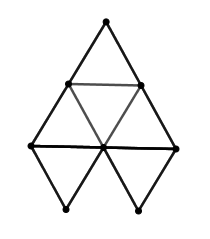
\includegraphics[width=50pt]{35.png}}
  
  %%%%%%%%%%%%%%%%%%%%%%%%%%%%%%%%%%%%%%%%%%%%%%
  
  \priklad{V protisměru se dva vlaky míjí po dobu 5 sekund. Pokud by se ovšem vlaky míjely při cestě stejným směrem, trvalo by to 15 sekund. Víme, že rychlejší vlak měří 600 metrů, zatímco pomalejší vlak měří dvojnásobek. Jaká je rychlost rychlejšího vlaku v metrech za sekundu?}{$ 240\,m/s $}
  
  %%%%%%%%%%%%%%%%%%%%%%%%%%%%%%%%%%%%%%%%%%%%%%%
  
  \priklad{Nekonečně velký papír má tloušťku $ 1\,mm $. Když ho rozpůlím a obě poloviny položím na sebe, bude mít takováto hromádka dvojnásobnou výšku. Pokud papír opět rozpůlím a položím na sebe, výška hromádky se opět zdvojnásobí. Jakou výšku bude mít hromádka po 30. přeložení?}{$ 2^{30}\,mm $}
  
  %%%%%%%%%%%%%%%%%%%%%%%%%%%%%%%%%%%%%%%%%%
  
  \priklad{Součet druhých mocnin tří jednociferných čísel se rovná číslu 105. Která čísla to jsou?}{4; 5; 8}
  
  %%%%%%%%%%%%%%%%%%%%%%%%%%%%%%%%%%%%%%%%%%%%%
  
  \priklad{8 šéfů gangu tvoří pouze $ 2{,}5\% $ ze všech jeho členů, ale rozdělili si $ 50\% $ celého pokladu. Kolikrát více pokladu získal šéf oproti řadovému členovi gangu?}{39krát}
  
  %%%%%%%%%%%%%%%%%%%%%%%%%%%%%%%%%%%%%%%%%%%
  
  \priklad{Máme 5 balíčků označených písmeny $ A $ až $ E $. Víme, že balíčky $ A $ a $ B $ váží dohromady $ 13\,kg $, $ B $ a $ C $ váží $ 12{,}5\,kg $. Balíky $ C $ a $ D $ pak mají $ 13{,}5\,kg $ a zásilky $ D $ a $ E $ váží $ 10\,kg $. Balíčky $ A $, $ C $ a $ E $ mají celkem $ 18\,kg $. Který balíček je nejtěžší a kolik váží?}{balíček $ A $, váží $ 7{,}5\,kg $}
  
  %%%%%%%%%%%%%%%%%%%%%%%%%%%%%%%%%%%%%%%%%%%%%%%
  
  \priklad{Ráno jsem vyšla z domu s jistým finančním obnosem. Jako první jsem ten den zašla na snídani, která mě stála 80 Kč. Pak jsem si koupila denní tisk za 25 Kč. Poté jsem potkala svou kamarádku, a protože byl krásný den, rozhodly jsem se, že si uděláme výlet. Koupila jsem nám tedy lístky na vlak, které mě stály polovinu peněz, které jsem v té době měla u sebe. V poledne jsme si zašly na výborný oběd, který mě stál 226 Kč. Odpoledne jsme strávily nákupy, kde jsem utratila dvě třetiny zbývajících financí. Zpáteční lístek mě ale naštěstí vyšel už jen na 108 Kč. Tři čtvrtiny toho, co mi ještě zbývalo, jsem pak použila na nákup potravin a posledních 20 Kč jsem věnovala na dobročinné organizaci těsně před tím, než jsem zašla do svého domu. S kolika penězi jsem ráno odcházela z domova?}{1685 Kč}
  
  %%%%%%%%%%%%%%%%%%%%%%%%%%%%%%%%%%%%%%%%%%
  
  \priklad{Mezi sedm sedmiček vložte sčítání tak, aby jejich součet byl 868.}{7+7+77+777}
  
  %%%%%%%%%%%%%%%%%%%%%%%%%%%%%%%%%%%%%%%%%
  
  \priklad{Jaký bude součet řady 2+4+6+8+10+12+14+16+18+...+2018.}{1019090}
  
  %%%%%%%%%%%%%%%%%%%%%%%%%%%%%%%%%%%%%%%%%%
  
  \priklad{Graf lineární funkce prochází body [-1;6] a [1;-2] . Určete předpis této funkce a spočítejte jeho průsečíky s~osami.}{$ y=-4x+2$, $ [0;2][\frac{1}{2};0] $}
  
  %%%%%%%%%%%%%%%%%%%%%%%%%%%%%%%%%%%%%%%%%%%%%
  
  \priklad{Ve stáji je sto boxů označených čísly od jedné do sta. V jednom boxu mužou být jeden, dva, nebo tři koně. Také víme, že v boxech 1 až 52 je dohromady 56 koní a v boxech 51 až 100 je celkem 150 koní. Kolik koní je dohromady ve stáji?}{200 koní}
  
  %%%%%%%%%%%%%%%%%%%%%%%%%%%%%%%%%%%%%%%%%%%%%%
  
  \prikladsobrazkem{Trojúhelníky $ABC$ a $KLM$ jsou vepsané kružnicím. Délky některých stran trojúhelníků jsou znázorněny na obrázku. Úsečky $AB$ a $KL$ prochází středy kružnic. Jakým číslem musíme vynásobit všechny délky stran trojúhelníku $KLM$, aby byl shodný s trojúhelníkem $ABC$?}{2/3}{46.png}{0.6}{0.4}
  
  %%%%%%%%%%%%%%%%%%%%%%%%%%%%%%%%%%%%%%%%%%%%%%%
  
  \priklad{Určete postupný poměr čtyř čísel $ a : b : c : d $ v základním tvaru, jestliže zároveň platí: $ b : d = 5 : 11 $ , $ a : b = 3 : 7 $ ,$  a : c = 2 : 9 $.}{30 : 70 : 135 : 154} 
  
  %%%%%%%%%%%%%%%%%%%%%%%%%%%%%%%%%%%%%%%%%%%
  
  \priklad{Za půl roku zaplatila domácnost $ x $ Kč za veškeré náklady spojené s elektrickou energií. Měsíční pronájem elektroměru byl přitom $ m $ Kč a $ 1\,kWh $ spotřebované elektrické energie stojí $ s $ Kč. Vyjádřete pomocí $ x $, $ m $ a $ s $, kolik $ kWh $ tato domácnost za dané období spotřebovala.}{$ (x - 6m)/s $}
  
  %%%%%%%%%%%%%%%%%%%%%%%%%%%%%%%%%%%%%%%%%%
  
  \priklad{Luděk, Marek a Norbert ztroskotali na pustém ostrově. Povedlo se jim naštěstí zachránit nějakou zásobu jídla. Luďkovi a Markovi by toto jídlo stačilo na 45 dní. Markovi a Norbertovi by tato zásoba stačila dokonce na 60 dní a Luďkovi s Norbertem by trvalo sníst všechno jídlo dokonce 90 dní. Jenže na ostrově jsou všichni tři, takže za jak dlouho jim dojde jídlo?}{za 40 dní}
  
  %%%%%%%%%%%%%%%%%%%%%%%%%%%%%%%%%%%%%%%%%%%
  
  \prikladsobrazkem{Trojúhelník je rozdělen na tři deltoidy (viz obrázek). Jaké jsou délky stran deltoidů $ x $, $ y $ a $ z $, když víme, že strany trojúhelníku mají délky 36, 50 a $ 54\,cm $?}{$ x = 16$ , $ y = 34$ , $ z = 20 $}{50.png}{0.6}{0.5}
  
  %%%%%%%%%%%%%%%%%%%%%%%%%%%%%%%%%%%%%%%%%%%
  
  \priklad{Eva má v bance 450 000 Kč, které se jí za rok zúročí o 3\%. Z úroků se ale musí odvádět státu 15\% daň. Kolik korun bude tedy tento rok odvedeno na daních?}{2 025 Kč}
  
  %%%%%%%%%%%%%%%%%%%%%%%%%%%%%%%%%%%%%%%%
  
  \priklad{Určete  nejmenší hodnotu proměnné $ a $ (z oboru reálných čísel), pro kterou platí: $$a + 1 = (\sqrt{ a + 5} - 2)( \sqrt{a + 5} + 2) $$}{-5}
  
  %%%%%%%%%%%%%%%%%%%%%%%%%%%%%%%%%%%%%%%%%%%
  
  \priklad{Pan Chroustal zapálil současně dvě svíčky jednou zápalkou. Pro tyto svíčky platí následující: Jedna z nich měřila $ 22\,cm $ a dohořela za 3 hodiny. Druhá, kratší a silnější, měřila původně $ 14\,cm $ a dohořela za 5 hodin. Určete, ve kterém okamžiku měly obě hořící svíčky stejnou délku. Výsledek zapište ve tvaru $ h\,mm\,ss $. Určete tuto délku s přesností na setiny $ cm $. Předpokládáme, že svíčky se zkracovaly rovnoměrně.}{$ 1\,h\,45\,min\,53\,s$,  délka je $9{,}06\,cm $}
  
  %%%%%%%%%%%%%%%%%%%%%%%%%%%%%%%%%%%%%%%%%%%%
  
  \priklad{Sečtěte  všechna čísla, která jsou násobkem 5 nebo 7 (nebo obojí) a jsou menší než 2018.}{$ 640\,487 $}
  
  %%%%%%%%%%%%%%%%%%%%%%%%%%%%%%%%%%%%%%%%%%%
  
  \priklad{Kvůli zlodějíčkům měli v obchodě průměrné ztráty ve výši $ 1{,}8\% $ průměrné denní tržby. Když si obchod najal hlídače, ztráty se snížily na $ 1{,}4\% $ průměrné denní tržby, ale protože denní náklady na hlídání byly 2000 Kč, obchodu se nevyplatil. Když si obchod najal hlídací firmu, ztráty se snížily na $ 0{,}6\% $ průměrné denní tržby. A to už se obchodu vyplatilo, i přesto, že hlídací firma stála denně 5 000 Kč. V jakém intervalu se tedy mohla pohybovat průměrná denní tržba tohoto obchodu?}{$ 416\,666{,}6 - 500\,000 $ Kč}
  
  %%%%%%%%%%%%%%%%%%%%%%%%%%%%%%%%%%%%%%%%%%%
  
  \priklad{Ljuba leží v posteli a přemítá, že by si k snídani udělala palačinky. Ale mají všechno potřebné doma? Mouka tam bude tak na 90\%, myslí si Ljuba. Ale s mlékem je to tak padesát na padesát a vsadím se, že ta dvě zbývající vajíčka si na sedmdesát procent dal brácha k snídani. Jak vysoká je pravděpodobnost, že si Ljuba palačinky k snídani opravdu udělá?}{$ 13{,}5\% = 27/200 $}
  
  %%%%%%%%%%%%%%%%%%%%%%%%%%%%%%%%%%%%%%%%%%%
  
  \priklad{Robert a Tadeáš se potřebují dostat do města vzdáleného $ 27\,km $ a chtějí tam dorazit oba dva zároveň. Problém je ale v tom, že mají jen jedno kolo a žádný jiný dopravní prostředek není k dispozici. Robert navrhl, že napřed pojede na kole, které na smluveném místě zanechá, a zbytek dojde pěšky. A Tadeáš půjde napřed pěšky a zbytek cesty pak pojede na kole. Robert umí chodit rychlostí $ 5\,km/h $, tedy o čtvrtinu rychleji než Tadeáš. Naopak Tadeáš je zase rychlejší na kole a to dokonce o $ 2\,km/h $, takže jezdí průměrnou rychlostí $ 10\,km/h $. V závislosti na tom si spočítali, kde si kolo nechají a vyrazili. Jakou nejkratší dobu jim tedy bude trvat cesta, když vyrazí i dorazí zároveň?}{$ 4{,}5\,h $}
  
  %%%%%%%%%%%%%%%%%%%%%%%%%%%%%%%%%%%%%%%%%%
  
  \priklad{Ve Lhotce si postavili vyhlídku, na kterou vedou zvláštní schody: první schod má výšku $ 42\,cm $ a každý další schod je o $ 0{,}5\,cm $ nižší. Poslední schod má pak $ 0,5\,cm $. Jaká je výška celého schodiště?}{$ 1785\,cm $}
  
  %%%%%%%%%%%%%%%%%%%%%%%%%%%%%%%%%%%%%%%%%%%%%
  
  \priklad{Tři bratři, Pankrác, Servác a Bonifác, mají narozeniny ve stejný den. O jedněch narozeninách si všimli, že součet věků dvou z nich je roven věku třetího. O několik let později (několik může být i 1) na jejich narozeniny platilo, že součet věků dvou z nich je roven dvojnásobku věku třetího z nich. A po čase, kdy od prvních zmíněných narozenin uplynula stejně dlouhá doba, jako jsou dvě třetiny ze součtu věků všech tří bratrů o prvních zmíněných narozeninách, bylo jednomu z trojice 28 let. Kolikáté narozeniny slavili ten den zbylí dva?}{20, 24}
  
  
  
  \end{enumerate}
  \end{document}
  